\documentclass[candidate, subf, href, colorlinks]{disser}
% Add `fixint` for straight integral signs

\usepackage [T2A] {fontenc}
\usepackage [utf8] {inputenc}
\usepackage [russian, english] {babel}
\usepackage {epstopdf}
\usepackage [autostyle] {csquotes}
\usepackage [intlimits] {amsmath}
\usepackage {amssymb, amsfonts}
\usepackage {amsthm}
\usepackage {hyperref}
\usepackage {array}
\usepackage {multicol}

% Margins
\usepackage[a4paper, mag=1000, left=2.5cm, right=1cm, top=2cm, bottom=2cm, headsep=0.7cm, footskip=1cm]{geometry}

\usepackage{wrapfig} % floating figures

\usepackage[style=gost-numeric, backend=biber, language=auto, hyperref=auto, autolang=other, sorting=none
]{biblatex}

\addbibresource{bibliography.bib} % bibliography source

% Page number position config
\pagestyle{footcenter}
\chapterpagestyle{footcenter}

% Definitions
\newtheorem{proposition}{Proposition}
\newtheorem{corollary}{Corollary}
\newtheorem{lemma}{Lemma}
\newtheorem*{lemma*}{Lemma}

\begin{document}

\institution{Московский институт электронной техники (МИЭТ)}

% UDC number
\libcatnum{519.6}

\author{Лебедев Михаил Евгеньевич}

\topic{\dots}

\specnum{05.13.18}
\spec{Математическое моделирование, численные методы и комплексы программ}

\title{ДИССЕРТАЦИЯ \\ на соискание ученой степени \\ кандидата физико-математических наук}

\sa{Г. Л. Алфимов}
\sastatus{д.~ф.-м.~н., проф.}

\city{Москва}
\date{\number\year}

\maketitle

% Content
\tableofcontents

% Introduction
\chapter*{Itroduction}
\addcontentsline{toc}{chapter}{Introduction}

One dimensional Gross--Pitaevskii equation (describes ``cigar-shaped'' condensate) takes form:
\begin{equation}
	i \Psi_t + \Psi_{xx} + U(x) \Psi + P(x) |\Psi|^2 \Psi = 0.
\label{eq:gross-pitaevskii}
\end{equation}

Here $\Psi(t, x)$ is the macroscopic wave function of the condensate, $U(x)$ corresponds to the potential of the trap holding the condensate, and $P(x)$ describes characteristic length of the atomic interactions.
Function $P(x)$ is called as {\it pseudopotential} which is induced by spatial periodic modulation.
This can be achieved in BEC by means of the Feshbach resonance controlled by magnetic or optical field \cite{PollackDriesJunkerChenCorcovilosHulet, ChinGrimmJulienneTsienga, BauerLetterVoRempeDurr}.
In the nonlinear optics spatial modulation of the Kerr coefficient can be induced by inhomogeneous density of resonant nonlinearity-enhancing dopants implanted into the waveguide \cite{HukriedeRundeKip}.

\dots

% Why real? All definitions! Stationary states equation.
% Energy and norm for the general case (U(x), P(x)).
 

% Literature review
% \input{review}

% TODO: Labels in the beginning, not in the end.
\chapter{General Propositions on Regular and Singular Solutions for Stationary States Equation $u_{xx} + Q(x) u + P(x) u^3 = 0$}
\label{chapter:I}

\section{Objectives}

In this chapter we formulate general statements about singular and regular solutions for the equation
\begin{equation}
	u_{xx} + Q(x) u + P(x) u^3 = 0.
	\label{eq:main}
\end{equation}
% TODO: Move this part to the introduction.
%As it was shown previously this equation follows from the original Gross--Pitaevskii equation by the the substitution
%\begin{equation}
%	\Psi(t, x) = u(x) e^{-i \omega t},
%\end{equation}
%where the corresponding localization conditions allow us to consider $u(x)$ as a real-valued function.
In general, we suppose that $Q(x), P(x) \in C^1(\mathbb{R})$ and will impose additional restrictions further when it's needed.
% TODO: Definitions of "regular / singular solution" and "collapse" must be presented in introduction.
Mainly we address two questions: (A) when do exist regular solutions of \eqref{eq:main}; (B) what are the conditions for the functions $Q(x)$ and $P(x)$ which can guarantee the existence of the singular solutions for equation \eqref{eq:main}; and (C) what is the behaviour of the collapsing solutions near the collapse point.
In this chapter partial answer to the question (A) is given by the Proposition~\ref{prop:absense-of-singular-solutions}.
On other hand Propositions~\ref{prop:singular-families} and \ref{prop:all-solutions-are-singular} give a partial answer to the question (B).
In particular Proposition~\ref{prop:singular-families} states that if the function $P(x)$ is negative at a point $x = x_0$ then there exist two one-parametric families of solutions collapsing at $x_0$.
Proposition~\ref{prop:singular-families} determines an asymptotic behaviour of these singular solutions families, which gives an answer to the question (C) for these families.

\section{Non-existence of Singular Solutions: $P(x) \ge P_0 > 0$}

This section contains a sufficient condition for non-existence of singular solutions for equation \eqref{eq:main}.
It's given by the following proposition.

\begin{proposition}
	Let functions $Q(x), P(x) \in C^1(\mathbb{R})$, moreover:
	\begin{enumerate}
		\item[(a)] $P(x) \ge P_0 > 0$, $|P'(x)| \le \widetilde{P}$;
		\item[(b)] $Q(x) \ge Q_0$, $|Q'(x)| \le \widetilde{Q}$;
	\end{enumerate}
	then solution of the Cauchy problem for equation \eqref{eq:main} with arbitrary initial conditions $u(x_0) = u_0$, $u_{x}(x_0) = u_0'$ can be continued to the whole real axis $\mathbb{R}$.
	\label{prop:absense-of-singular-solutions}
\end{proposition}
\begin{proof}
	By the existence and uniqueness theorem for ODE there exists an interval $[x_0; x_1)$ such that the solution of the Cauchy problem $u(x)$ for equation \eqref{eq:main} with initial conditions $u(x_0) = u_0$, $u_{x}(x_0) = u_0'$ exists and is unique on this interval, and $u(x) \in C^2[x_0; x_1)$.
	Suppose that $[x_0; x_1)$ is the maximum interval for existence of $u(x)$.
	It means that solution of the Cauchy problem $u(x)$ cannot be continued beyond the point $x_1$.
	Multiplying the original equation by $4u_{x}(x)$ and integrating it over $[x_0, x)$, $x < x_1$, we have the following relation:
	\begin{equation}
	\begin{aligned}
		& 2 u_x^2(x)) + 2 Q(x) u^2(x) - 2 \int \limits_{x_0}^{x} Q'(\xi) u^2(\xi) d\xi + P(x) u^4(x) - \int \limits_{x_0}^x P'(\xi) u^4(\xi) d\xi = \\
		& \quad = 2 (u_0')^2 + 2 Q(x_0) u_0^2 + P(x_0) u_0^4 \equiv C.
		\label{eq:aux-04}
	\end{aligned}	
	\end{equation}
	Omit the term $u_{x}^2(x) \ge 0$ in the left-hand side of the equality, and take into account the lower limits for $Q(x)$, $P(x)$ given by conditions (a), (b).
	Then we arrive at the following inequality:
	\begin{equation}
		2 Q_0 u^2(x) + P_0 u^4(x) \le C + 2 \int \limits_{x_0}^{x} Q'(\xi) u^2(\xi) d\xi + \int \limits_{x_0}^{x} P'(\xi) u^4(\xi) d\xi.
	\end{equation}
	Replace the derivatives $Q'(\xi)$ and $P'(\xi)$ with their upper bounds: $Q'(\xi) \le \widetilde{Q}$, $P'(\xi) \le \widetilde{P}$, where $\widetilde{Q} \ge 0$, $\widetilde{P} \ge 0$.
	Multiplying both sides of the inequality by $P_0$, we have
	\begin{equation}
		2 Q_0 P_0 u^2(x) + P_0^2 u^4(x) \le P_0 C + 2 P_0 \widetilde{Q} \int \limits_{x_0}^{x} u^2(\xi) d\xi + P_0 \widetilde{P} \int \limits_{x_0}^{x} u^4(\xi) d\xi.
		\label{eq:aux-01}
	\end{equation}
	Let $v(x) = (P_0 u^2(x) + Q_0)^2$, $v(x) \ge 0$, substituting this into \eqref{eq:aux-01} gives
	\begin{equation}
		v(x) \le \widetilde{C} + \dfrac{\widetilde{P}}{P_0} \int \limits_{x_0}^{x} w(v(\xi)) d\xi.
		\label{eq:aux-02}
	\end{equation}
	Here $\widetilde{C} = P_0 C + Q_0^2 \ge 0$, $\alpha = 2 \widetilde{Q} P_0 / \widetilde{P} \ge 0$, and $w(v)$ is defined by
	\begin{equation}
		w(v) \equiv \alpha (\sqrt{v} - Q_0) + (\sqrt{v} - Q_0)^2.
	\end{equation}
	Consider the function
	\begin{equation}
		G(s) = \int \limits_{s_0}^{s} \dfrac{dv}{w(v)}.
	\end{equation}
	Here $s_0 > Q_0^2$ is an arbitrary constant, $s \ge s_0$.
	Since $w(v)$ is a positive and monotonically decreasing function, and the integral
	\begin{equation}
		\int \limits_{s_0}^{+\infty} \dfrac{dv}{w(v)}
	\end{equation}
	diverges, one can conclude that $G(s)$ is a positive, monotonically increasing, and unbounded function.
	It means that inverse function $G^{-1}(r)$ is well-defined for $r \ge 0$, increases monotonically, and is unbounded.
	The above-mentioned statements allow as to apply {\it Bihary} inequality \cite[theorem 2.3.1]{Pachpatte} to \eqref{eq:aux-02}.
	This results in the inequality
	\begin{equation}
		v(x) \le G^{-1} \left( G(\widetilde{C}) + \dfrac{\widetilde{P}}{P_0} \int \limits_{x_0}^{x} d\xi \right) = G^{-1} \left( G(\widetilde{C}) \dfrac{\widetilde{P}}{P_0} (x - x_0) \right) < \infty.
		\label{eq:bihari}
	\end{equation}
	Inequality \eqref{eq:bihari} is valid for all $x \in [x_0; x_1)$.
	It follows from \eqref{eq:bihari} that function $v(x)$ is bounded on the whole interval $[x_0; x_1)$:
	\begin{equation}
		v(x) \le M = G^{-1} \left( G(\widetilde{C}) + \dfrac{\widetilde{P}}{P_0} (x_1 - x_0) \right).
	\end{equation}
	We observe that $\widetilde{C} \ge Q_0^2$, moreover $\widetilde{C} = Q_0^2$ only if $u_0 = u_0' = 0$.
	It means that $G(s)$ is well-defined for each constant $\widetilde{C}$ corresponding to any non-zero solution $u(x)$.
	The boundedness of $v(x)$ yields that solution $u(x)$ is also bounded on the segment $[x_0; x_1)$:
	\begin{equation}
		|u(x)| \le \sqrt{\dfrac{\sqrt{M} - Q_0}{P_0}}, \quad x \in [x_0; x_1).
		\label{eq:aux-03}
	\end{equation}
	Substitution of \eqref{eq:aux-03} into \eqref{eq:aux-04} gives the upper bound for the derivative $u_{x}(x)$ on the interval $x \in [x_0; x_1)$.
	Since functions $u(x)$ and $u_{x}(x)$ are continuous and bounded on $[x_0; x_1)$, the values $u(x_1) = u_1$ and $u_{x}(x_1) = u_1'$ are finite.
	Hence there exists a continuation of the solution to the Cauchy problem with the initial conditions $u(x_0) = u_0$, $u_{x}(x_0) = u_0'$ on a larger interval beyond the initial $[x_0; x_1)$.
	It contradicts the original assumption.
	
	Thus we have proved that the solution can be continued for $x > x_0$.
	In order to prove the same statement for $x < x_0$, one can make a substitution $x \to -x$ and employ the same reasoning.
\end{proof}

\begin{corollary}
	If the conditions (a) and (b) are satisfied not on the whole real axis $\mathbb{R}$, but only on some interval $[x_1; x_2]$, then a solution of the Cauchy problem for equation \eqref{eq:main} with arbitrary initial conditions does not collapse at any point of the segment $[x_1; x_2]$.
\end{corollary}

\section{Asymptotic Behaviour at a Collapse Point: $P(x_0) < 0$}

\subsection{Asymptotic Expansions}

If $P(x)$ is negative at least at one point $x_0 \in \mathbb{R}$, formal asymptotic expansions predict existence of two one-parametric families of the solutions for the equation \eqref{eq:main} collapsing at this point.

Let us construct these asymptotic expansions.
We suppose that $P(x_0) = -1$ (this condition can be achieved by a simple renormalisation of the independent variable), denote $\eta = x - x_0$, and assume that in the vicinity of the point $x = x_0$, the following expansions are valid:
\begin{equation}
	Q(x) = Q_0 + Q_1 \eta + Q_2 \eta^2 \dots, \quad P(x) = -1 + P_1 \eta + P_2 \eta^2 + \dots.
\end{equation}
Substituting these expansions into \eqref{eq:main}, we have
\begin{equation}
	u_{\eta\eta} + (Q_0 + Q_1 \eta + Q_2 \eta^2 \dots)u + (-1 + P_1 \eta + P_2 \eta^2 + \dots) u^3 = 0.
	\label{eq:aux-11}
\end{equation}
If a solution $u(\eta)$ of equation \eqref{eq:aux-11} collapses at the point $\eta = 0$ then $u(\eta) \to \pm \infty$, when $\eta \to 0$.
Let $\eta$ approach zero {\it from the right}, $\eta > 0$.
The change $v(\eta) = \eta u(\eta)$, $\eta = e^{-t}$ gives
\begin{equation}
	v_{tt} + 3v_{t} + 2v + e^{-2t} Q(t) v + P(t) v^3 = 0.
	\label{eq:asymptotic-problem}
\end{equation}
Determine the main term of the expansion by balancing $2v$ and $-v^3$ terms.
We have
\begin{equation}
	V_0(t) = \pm \sqrt{2}.
	\label{eq:main-term}
\end{equation}
Now let's define the first order term $V_1(t)$, $v(t) = \pm \sqrt{2} + V_1(t) + o(V_1(t))$.
Substituting the last expression into \eqref{eq:asymptotic-problem}, taking into account the expansions for the functions $Q(t)$, $P(t)$, and omitting the terms of order higher than $e^{-t}$, we obtain
\begin{equation}
	V_{1, tt} + 3V_{1, t} - 4V_1 = \mp 2 \sqrt{2} e^{-t},
\end{equation}
that gives $V_1(t) = \pm \frac{\sqrt{2}}{3} e^{-t}$.
Second, third, and forth order terms $V_n$, $n = 2, 3, 4$, can be found in a similar manner.
For each term the corresponding equation takes form:
\begin{equation}
	V_{n, tt} + 3V_{n, t} - 4V_n = C_n e^{-nt}.
	\label{eq:high-order-terms-equation}
\end{equation}
For $n = 2, 3$ solutions of equation \eqref{eq:high-order-terms-equation} are of the form $V_n \sim e^{-nt}$.
However in the case $n = 4$ the exponent degree in the right hand side coincides with one of the roots of the characteristic polynomial for the differential operator in the left-hand side.
In this case solution of equation \eqref{eq:high-order-terms-equation} must be chosen in the form $Ce^{-4t} - A_3 t e^{-4t}$.
Here $C$ in an arbitrary constant, while $A_3$ can be determined uniquely from the coefficients of the series expansions for $Q(t)$, $P(t)$.
If constant $C$ is fixed, at the further steps of this procedure the corresponding equations are uniquely solvable.
One can note that switching of $+$ to $-$ in the expression \eqref{eq:main-term} leads to the corresponding change of signs for all coefficients $A_n$, $n = 0, 1,...$, that is natural due to the invariance of equation \eqref{eq:main} with respect to the change $u \to -u$.
We have
\begin{equation}
	\pm v(t) = \sqrt{2} + A_0 e^{-t} + A_1 e^{-2t} + A_2 e^{-3t} + A_3 \cdot (-t) \cdot e^{-4t} + C e^{-4t} + \dots.
	\label{eq:expansion-intermediate}
\end{equation}
Explicit expressions for $A_0, \dots, A_3$ are:
\begin{eqnarray}
	& A_0 & = \dfrac{\sqrt{2}}{3} P_1; \label{eq:aux-A0} \\
	& A_1 & = \dfrac{\sqrt{2}}{3} P_2 + \dfrac{\sqrt{2}}{6} Q_0 + \dfrac{2 \sqrt{2}}{9} P_1^2; \label{eq:aux-A1} \\
	& A_2 & = \frac{2\sqrt{2}} 3P_2 P_1 + \frac{7\sqrt{2}}{27} P_1^3 + \frac{\sqrt{2}} 6Q_0 P_1 + \frac{\sqrt{2}} 4Q_1 + \frac{\sqrt{2}} 2P_3; \label{eq:aux-A2} \\
	& A_3 & = -\dfrac{\sqrt{2}}{6} Q_1 P_1 - \dfrac{\sqrt{2}}{5} Q_2 - \dfrac{32 \sqrt{2}}{45} P_2 P_1^2 - \dfrac{3 \sqrt{2}}{5} P_3 P_1 - \\
	&& - \dfrac{2 \sqrt{2}}{15} P_2 Q_0 -\dfrac{2 \sqrt{2}}{15} Q_0 P_1^2 - \dfrac{2 \sqrt{2}}{5} P_4 - \dfrac{28 \sqrt{2}}{135} P_1^4 - \dfrac{4 \sqrt{2}}{15} P_2^2. \label{eq:aux-A3}
\end{eqnarray}

In the other case when $\eta \to 0$ {\it from the left}, $\eta < 0$, similar expansions can be constructed by mean of changes of variables $v(\eta) = \eta u(\eta)$, $\eta = -e^{-t}$.
Expressions for the coefficient $A_n$ remain the same as for $\eta > 0$.

Finally we get an asymptotic expansion for the original solution $u(x)$ for $x \to x_0 \pm 0$:
\begin{equation}
	\pm u(x) = \dfrac{\sqrt{2}}{\eta} + A_0 + A_1 \eta + A_2 \eta^2 + A_3 \eta^3 \ln |\eta| + C \eta^3+ A_4 \eta^4 \ln |\eta| + \dots.
	\label{eq:expansion}
\end{equation}
Here $\eta = x - x_0$, $A_0, \dots, A_3$ are determined by equations \eqref{eq:aux-A0}-\eqref{eq:aux-A3}, and all other coefficients $A_n$, $n > 3$ can be expressed through $Q_n$, $P_n$ and arbitrary constant $C$.

Summarizing all the above mentioned, one can say that asymptotic expansion \eqref{eq:expansion} {\it predicts the existence} of two one-parametric families of solutions collapsing at the point $x_0$.
These families are connected by the symmetry $u \to -u$.
When $x \to x_0$, the solutions from one of these families tend to $+\infty$, while the solutions from another family tend to $-\infty$ correspondingly.

\subsection{Existence of One-Parametric Families of Collapsing Solutions}

Strictly speaking, formal asymptotic expansions \eqref{eq:expansion} do not imply the existence of one-parametric families of solutions collapsing at point $x_0$.
However, the following rigorous statement holds.

\begin{proposition}
	Let $\Omega$ be a neighbourhood of the point $x_0$, $Q(x) \in C^2(\Omega)$ and $P(x) \in C^4(\Omega)$.
	Then there exist two $C^1$-smooth one-parametric families of solutions for equation \eqref{eq:main} corresponding to expansions \eqref{eq:expansion}, collapsing at the point $x = x_0$ (while approaching from the left, $x < x_0$), and connected by a symmetry $u \to -u$.
	Each of these families can be parametrized by a free variable $C \in \mathbb{R}$ from the expansions \eqref{eq:expansion}.
\label{prop:singular-families}
\end{proposition}
\begin{proof}
	Due to the condition of proposition the following expansions are valid:
	\begin{eqnarray}
		& Q(x) & = Q_0 + Q_1 \eta + Q_2 \eta^2 + \widetilde{Q}(\eta) \eta^3; \\
		& P(x) & = -1 + P_1 \eta + P_2 \eta^2 + P_3 \eta^3 + P_4 \eta^4 + \widetilde{P}(\eta) \eta^5.
	\end{eqnarray}
	Here $\eta = x - x_0$, and $\widetilde{Q}, \widetilde{P} \in C(\Omega)$.
	To prove existence of the family that corresponds to the $+$ sign in \eqref{eq:expansion}	 we introduce the function $z(\eta)$ as follows:
	\begin{equation}
		u(x) = \dfrac{\sqrt{2}}{\eta} + A_0 + A_1 \eta + A_2 \eta^2 + A_3 \eta^3 \ln(-\eta) + z(\eta) \eta^3,
		\label{eq:aux-20}
	\end{equation}
	($z(\eta)$ is a new unknown function).
	Coefficients $A_0, \dots, A_3$ are chosen accordingly to the expressions \eqref{eq:aux-A0}-\eqref{eq:aux-A3}, so the coefficients at the terms $\eta^{-2}$, $\eta^{-1}$, $\eta^0$, and $\eta$ vanish.
	It's easy to check that direct substitution of the \eqref{eq:aux-20} into \eqref{eq:main} yields
	\begin{equation}
		z_{\eta\eta} + \dfrac{6}{\eta} z_{\eta} + g(\eta, z) = 0,
		\label{eq:aux-z}
	\end{equation}
	where $g(\eta, z)$ is a third order polynomial with respect to $z$, and $g(\eta, z) \sim \frac{\ln(-\eta)}{\eta}$ when $\eta \to -0$ and $z$ is fixed.
	The change of variable $\eta = -e^{-t}$ maps the point $\eta = 0$ into $t = +\infty$, and transforms equation \eqref{eq:aux-z} into
	\begin{equation}
		z_{tt} - 5z_t - f(t, z) = 0.
		\label{eq:aux-zt}
	\end{equation}
	Here $f(t, z) \sim t e^{-t}$ while $t \to +\infty$.
	Properties of the function $f(t, z)$ allows us to apply {\it Lemma on Bounded Solutions} from Appendix \ref{appendix:lemma-on-bounded-solutions} to equation \eqref{eq:aux-zt}.
	This lemma states that for $t \to +\infty$ all bounded solutions of equation \eqref{eq:aux-zt} tend to some constant $C$ when $t \to +\infty$, moreover for each $C \in \mathbb{R}$ there exists a unique solution that approaches to that constant asymptotically while $t \to +\infty$.
	Furthermore these solutions form a $C^1$-smooth family.
	Finally, we can return to previous equation \eqref{eq:aux-z}, and then to \eqref{eq:main} to get the initial statement of the proposition.
	The existence of the second family of solutions corresponding to the sign ``$-$'' in \eqref{eq:expansion} follows from the invariance of equation \eqref{eq:main} under the symmetry $u \to -u$.
\end{proof}

Similar one-parametric families of collapsing solutions exist from the right side of the point $x = x_0$.
The corresponding proof can be performed in the same way.

\section{All Solutions Are Singular: $P(x) \le P_0 < 0$, $Q(x) \le Q_0 < 0$}

It turns out that under some assumptions all non-trivial solutions of the equation \eqref{eq:main} are singular.
\begin{proposition}
\label{prop:all-solutions-are-singular}
	Let for $x \in \mathbb{R}$ the conditions $P(x) \le P_0 < 0$, $Q(x) \le Q_0 < 0$ take place.
	Then all solutions of equation \eqref{eq:main} are singular except for the zero one.
\end{proposition}

To prove this proposition we prove the following auxiliary lemma first.
\begin{lemma}
	Let $p, q > 0$ are real constants, then all solutions of equation
	\begin{equation}
		v_{xx} - q v - p v^3 = 0,
		\label{eq:aux-lemma}
	\end{equation}
	are singular except for the zero one.
\end{lemma}
\begin{proof}
	The solution of the Cauchy problem for equation \eqref{eq:aux-lemma} with initial conditions $v(x_0) = v_0$, $v_x(x_0) = v_0'$ can be written in an implicit form as follows:
	\begin{equation}
		\pm \int \limits_{v_0}^{v} \dfrac{d\xi}{\sqrt{C + q \xi^2 + \dfrac{p}{2} \xi^4}} = x - x_0;	\quad C \equiv (v_0')^2 - q v_0^2 - \dfrac{p}{2} v_0^4.
		\label{eq:aux-21}
	\end{equation}
	Choice of the sign in the left hand-side depends on the initial conditions and the value of $x$.
	Integral in the left hand-side of the equality \eqref{eq:aux-21} converges when $v \to \infty$, and hence there exist a value $x^*$,
	\begin{equation}
		x^* = x_0 \int \limits_{v_0}^{\infty} \dfrac{d\xi}{\sqrt{C + q \xi^2 + \dfrac{p}{2} \xi^4}},
	\end{equation}
	such that $v(x)$ goes to infinity while $x$ approaches to the $x^*$ 
	So a solution $v(x)$ with arbitrary non-zero initial conditions is singular, lemma is proved.
\end{proof}

Now we can prove the Proposition 3.
\begin{proof}[Proof of the Proposition 3.]
	We use a so-called {\it Comparison Lemma} from \cite[Appendix C]{AlfimovZezyulin}.
	Consider the equation
	\begin{equation}
		v_{xx} + Q_0 v + P_0 v^3 = 0.
	\end{equation}
	We introduce the notations
	\begin{eqnarray}
		& g(x, \xi) & = -Q(x) \xi - P(x) \xi^3; \\
		& f(x, \xi) = f(\xi) & = -Q_0 \xi - P_0 \xi^3.
	\end{eqnarray}
	Now we apply Comparison Lemma to the following pair of equations:
	\begin{eqnarray}
		&& u_{xx} = g(x, u) \label{eq:comparison-u}; \\
		&& v_{xx} = f(x, v) \label{eq:comparison-v}.
	\end{eqnarray}
	In the domain $D_+ = \{ x \in \mathbb{R}, \xi \in (0; +\infty) \}$ we have $f(x, \xi) \le g(x, \xi)$.
	Let $\widetilde{u}(x)$ be a solution of the Cauchy problem for equation \eqref{eq:comparison-u} with initial conditions $u(x_0) = u_0$, $u_x(x_0) = u_0'$.
	Chose the initial conditions for the Cauchy problem for equation \eqref{eq:comparison-v} as follows: $v(x_0) = u(x_0) = u_0$, $v_x(x_0) = u_x(x_0) = u_0'$; let $\widetilde{v}(x)$ be a solution for that problem.
	Let $u_0 > 0$, then one of the two cases takes place.
	\begin{enumerate}
		\item[(i)] $u_0' \ge 0$.
		Function $\widetilde{v}(x)$ increases monotonically; this fact can be easily established from the phase portrait of equation \eqref{eq:comparison-v}.
		Solution $\widetilde{u}(x)$ bounds the solution $\widetilde{v}(x)$ from above.
		But $\widetilde{v}(x)$ is singular.
		Then it follows from Comparison Lemma that solution $\widetilde{u}(x)$ is also singular.
		\item[(ii)] $u_0' < 0$.
		We make a change of variable $\widetilde{x} = -x$.
		In that case solution $\widetilde{v}(\widetilde{x})$ also increases monotonically, and since $\widetilde{u}(\widetilde{x})$ limits $\widetilde{v}(\widetilde{x})$ from above, $\widetilde{u}(\widetilde{x})$ is singular by Comparison Lemma, hence $\widetilde{u}(x)$ is also singular.
	\end{enumerate}
	Similarly in the domain $D_- = \{ x \in \mathbb{R}, \xi \in (-\infty; 0) \}$, the inequality $f(x, \xi) \ge g(x, \xi)$ holds.
	One can prove in the same manner that in the domain $D_-$ solution $u(x)$ is also singular.
\end{proof}

\section{Summary}

Our main findings on regular and singular solutions for the stationary states equation \eqref{eq:main} are summarised in Table \ref{tab:first-chapter-results}.
Our further findings are focused on the case when $P(x)$ changes its sign.
In the next chapter we describe a so-called {\it method of excluding of singular solutions} which allows us to classify all regular solutions of equation \eqref{eq:main} within the symbolic dynamics framework.

\begin{table}[h!]
	\centering
	\begin{tabular}{ | p{4cm} | l || p{10cm} | }
		\hline
		$P(x)$ & $Q(x)$ & \\
		\hline
		$P(x) > 0$ & --- & All the solutions can be continued to the whole real line, singular solutions do not exist (Proposition~\ref{prop:absense-of-singular-solutions}). \\
		\hline
		$P(x) < 0$ at least at one point $x = x_0$ & --- & There exists a pair of one-parametrical families of solutions collapsing at point $x = x_0$ and related by the symmetry $u \to -u$ (Proposition~\ref{prop:singular-families}). \\
		\hline
		$P(x) < 0$ & $Q(x) < 0$ & All solutions are singular except for the zero one (Proposition~\ref{prop:all-solutions-are-singular}). \\
		\hline
		$P(x)$ changes sign along $\mathbb{R}$ & --- & Singular solutions are generic.
		That fact allows to apply the so-called {\it method of excluding of singular solutions} and classify all regular solutions in terms of symbolic dynamics.
		We describe this method and its application in Chapter~\ref{chapter:II}. \\
		\hline
	\end{tabular}
	\caption{
		Summary of the results for the Chapter 1.
		The results of this Chapter were published in \cite{AlfimovLebedev}.
	}
	\label{tab:first-chapter-results}
\end{table}


% Conclusion
% \chapter*{Conclusion}
\addcontentsline{toc}{chapter}{Conclusion}
\label{conclusion}

In the present work one-dimensional stationary states of Bose--Einstein condensate cloud were studied.
Dynamics of the condensate in so-called mean-field ap­proximation is well described by the Schr\"odinger type equation \eqref{eq:intro-gpe} with spatial non-au­tonomous terms.
One of this term, $U(x)$, corresponds to the potential that is used to confine condensate.
Another term, $P(x)$, called pseudopotential, describes the dependence of scattering length on the coordinates that can be made non-constant by various experimental techniques, such as Feshbach resonance.

In our study we focused on special subclass of the solutions, so-called stationary localized modes, SLMs, satisfying the ansatz \eqref{eq:intro-ansatz} and the localization conditions \eqref{eq:intro-localization}.
The profile of the stationary solutions is described by equation \eqref{eq:intro-stationary}.
Our goal was to identify stationary solutions for equation \eqref{eq:intro-gpe} and study their stability.
To describe stationary solutions for the case of both periodic potential and pseudopotential functions we developed a symbolic dynamics approach.
It allows under certain conditions to describe the solutions of equation \eqref{eq:intro-stationary} in terms of bi-infinite symbolic sequences, so-called codes.
Based on the structure of coding sets $\mathscr{U}_L^{\pm}$, which are the Poicar\'e map domains for equation \eqref{eq:intro-stationary}, one can assign a symbolic code to each stationary solution.
Besides, under specified conditions such correspondence is bijective.
This approach was applied to the cases of piecewise and cosine-form pseudopotential.
It turns out that there exists plethora of localized solutions in this model.
For cosine-form pseudopotential our comprehensive study revealed new types of stable solutions.

For the case of harmonic potential trap and periodic pseudopotential family of SLMs was also studied.
Since harmonic potential is not periodic, coding approach cannot be applied to such problem.
Numerical analysis showed that presence of periodic pseudopotential significantly enriches the family of localized solutions.
We also studied stability of low-amplitude localized solutions with asymptotic methods and describe the effect of the frequency of pseudopotential on their stability.
Stability of found stationary localized solutions was studied numerically with spectral method and confirmed by numerical simulation with finite-difference scheme.

Let's summarize in details main results of the thesis.
\begin{enumerate}
	\item The statements about the presence and absence of singular solutions of equation \eqref{eq:intro-stationary} are formulated and proved.
		It is shown that in the case $P(x) > 0$ all solutions of \eqref{eq:intro-stationary} are regular.
		If $P(x)$ is negative at the point $x_0$, $P(x_0) < 0$, then there exist two one-parametric families of solutions, which tend to infinity at the point $x_0$.
		In the case $Q(x) < 0$ and $P(x) < 0$, it is shown that all solutions of equation \eqref{eq:intro-stationary} are singular.
	\item An approach of one-to-one coding of solutions for equation \eqref{eq:intro-stationary} with periodic functions $Q(x)$, $P(x)$ has been developed.
		This approach requires some conditions to be met.
		These conditions are formulated in a form of two hypothesis and an efficient algorithm for their numerical verification is provided.
	\item For the case $U(x) \equiv 0$, $P(x) = A + \cos 2x$ the set of stationary localized modes for equation \eqref{eq:intro-gpe} has been studied.
		A new stable previously unknown solution, called {\it dipole soliton}, was found.
	\item In the case of harmonic potential well it was shown that including of periodic pseudopotential results in new classes of SLMs without linear counterpart.
		For the pseudopotential with zero mean, it was concluded that the increase of pseudopotential frequency stabilize low-amplitude solutions.
\end{enumerate}

In conclusion, let's also consider possible directions in which the current work can be further developed and generalized.
One of such directions is to consider a model described by GPE \eqref{eq:intro-gpe} for both periodic potential and periodic pseudopotential with different spatial frequencies.
Our coding approach can be applied to such case.
It's interesting to study family of stationary localized solutions and their stability in a view of interplay between these two spatial frequencies.

Another generalization of this study is related to two component BEC models \cite{TrippenbachGoralRzazewskiMalomedBand, OhbergSantos, SvidzinskyChui, NavarroCarreteroGonzalezKevrekidis, KevrekidisFrantzeskakis2016}.
These models describe mixtures of ultracold atoms of two different types.
It would be interesting to extend the methods developed in this work by considering four-dimensional plane of initial data and analysing counterparts of coding sets in this case. 
This study may result in classification of vector solitons admitted by the system under given parameters.
The next step of this perspective research would be the analysis of their stability.
It may be promising, since it was shown that including nonlinear lattice in one component of the two component model may stabilize two-dimensional vector solitons \cite{BorovkovaMalomedKartashov}.
Following the setup of the last paper, it would be quite interesting to extend the approach developed in this work to multidimensional problems.


\appendix
\renewcommand\thechapter{\Alph{chapter}}

\chapter{Lemma on Bounded Solutions}
\label{appendix:lemma-on-bounded-solutions}

\begin{lemma*}[On bounded solutions]
	Let $f(t, z)$ be a function that is continuous with respect to $t$ and continuously differentiable with respect to $z$.
	Let $f(t, z)$ is defined for $t \ge t_0$, $|z| < +\infty$, and have the following properties:
	\begin{itemize}
		\item[(i)] for $|z| < \rho$, $\rho > 0$, the estimate $|f(t, z)| < \eta_{\rho}(t)|z|$ is valid, where $\eta_{\rho}(t) \in L_1(t_0; +\infty)$;
		\item[(ii)] for all $z_1$, $z_2$ such that $|z_{1,2}| < \rho$, $\rho > 0$, there exists function $\tilde{\eta}_{\rho}(t) \in L_1(t_0; +\infty)$, such that $|f(t, z_2) - f(t, z_1)| \le \tilde{\eta}_{\rho}(t) |z_2 - z_1|$;
		\item[(iii)] for $|z| < \rho$, $\rho > 0$, the estimate $|f_z(t, z)| < \theta_{\rho}(t) |z|$ is valid, where $\theta_{\rho} \in L_1(t_0, +\infty)$;
		\item[(iv)] for all $z_1$, $z_2$ such that $z_{1,2} < \rho$, $\rho > 0$, there exists function $\tilde{\theta}_{\rho} \in L_1(t_0; +\infty)$, such that $|f_z(t, z_2) - f_z(t, z_1)| \le \tilde{\theta}_{\rho} |z_2 - z_1|$.
	\end{itemize}
	Then for the equation
	\begin{equation}
		z_{tt} - \alpha z_t + f(t, z) = 0, \quad \alpha > 0
		\label{eq:lemma-bs-main}
	\end{equation}
	the following statements are valid:
	\begin{itemize}
		\item[(A)] for each solution $z(t)$ of the equation \eqref{eq:lemma-bs-main} that is bounded when $t \to +\infty$ there exists $C \in \mathbb{R}$ such that $z(t) \to C$ as $t \to +\infty$;
		\item[(B)] for each $C \in \mathbb{R}$ there exists unique solution $Z(t, C)$ of the equation \eqref{eq:lemma-bs-main}, defined on a segment $(t_C; +\infty)$, such that
		\begin{equation}
			Z(t, C) = C + o(1), \quad t \to +\infty;
		\end{equation}
		\item[(C)] family of solutions $Z(t, C)$ is $C^1$-smooth with respect to the parameter $C$.
	\end{itemize}
\end{lemma*}
\begin{proof}
	Let us prove the statement (A) first.
	With the method of variation of parameters one can find that a solution of the equation \eqref{eq:lemma-bs-main} satisfies the equality:
	\begin{equation}
		z(t) = \varkappa_1 + \varkappa_2 e^{\alpha t} + \int \limits_{t_0}^{t} e^{\alpha \eta} \left( \int \limits_{\eta}^{+\infty} e^{-\alpha \xi} f(\xi, z(\xi)) d\xi \right) d\eta.
	\end{equation}
	It follows from the condition (i) that if $z(t)$ is bounded while $t \to +\infty$ then the integral
	\begin{equation}
		\int \limits_{t_0}^{+\infty} e^{\alpha \eta} \left( \int \limits_{\eta}^{+\infty} e^{-\alpha \xi} f(\xi, z(\xi)) d\xi \right) d\eta
	\end{equation}
	converges.
	Furthermore for all bounded solutions $\varkappa_2 = 0$, hence $z(t)$ tends to some constant for $t \to +\infty$.
	That proves the point (A).
	
	Move on to the point (B).
	We make a variable change $u(t) = z(t) - C$, where $C$ is an arbitrary number.
	Rewrite the equation \eqref{eq:lemma-bs-main} in the form of a system of equations
	\begin{equation}
		y_t = Ay + F(t, y),
		\label{eq:lemma-bs-system}	
	\end{equation}
	where
	\begin{equation*}
		y = \begin{pmatrix}
			u \\ v
		\end{pmatrix}, \quad
		A = \begin{pmatrix}
			0 & 1 \\
			0 & \alpha
		\end{pmatrix}, \quad
		F(t, y) = \begin{pmatrix}
			0 \\ f(t, u + C)
		\end{pmatrix}.
	\end{equation*}
	Now we apply Theorem 9.1 from \cite[Chapter XII]{Hartman} to the system \eqref{eq:lemma-bs-system}.
	It states that the system \eqref{eq:lemma-bs-system} {\it has a solution which tends to zero at infinity} \underline{if} the following conditions are satisfied:
	\begin{itemize}
		\item[(1)] function $F(t, y)$ is continuous and $||F(t, y)|| \le \lambda(t)$ for $t \in [t_0; +\infty)$, $||y|| \le \rho$, where $\lambda(t) \in L_1(t_0; +\infty)$;
		\item[(2)] for all $g(t) = col(g_1(t), g_2(t))$, $g(t) \in L_1(t_0; +\infty)$ there exists a solution $y(t) \in L_0^{\infty}(t_0; +\infty)$ of the inhomogeneous system
		\begin{equation}
			y_t = Ay + g(t);
			\label{eq:lemma-bs-hartman}
		\end{equation}
		(hereinafter by the norm $||\cdot||$ we mean the Euclidean norm in $\mathbb{R}$).
	\end{itemize}
	
	At first, by the condition (i) if $|u| \le \rho$ and $t > t_0$ relation $||f(t, u, C)|| \le \rho \eta_{\rho} (t)$ takes place, moreover $\eta_{\rho} \in L_1(t_0; +\infty)$, hence the condition (1) of the above-mentioned theorem is satisfied.
	At second, general solution of the inhomogeneous system of equations \eqref{eq:lemma-bs-hartman} can be written as:
	\begin{eqnarray}
		&& u(t) = C_2 + \int \limits_{t_0}^{t} \left( g_1(\eta) + e^{\alpha \eta} \left( C_1 - \int \limits_{+\infty}^{\eta} e^{-\alpha \xi} g_2(\xi) d\xi \right) \right) d\eta; \\
		&& v(t) = u_t(t) - g_1(t).
	\end{eqnarray}
	Since $g_{1,2}(t) \in L_1(t_0; +\infty)$ one can choose appropriate parameters $C_1$, $C_2$ in order to get a solution which tends to zero while $t \to +\infty$, so the condition (2) of the theorem is also met.
	Thereby both of the conditions for the applied theorem take place for the system \eqref{eq:lemma-bs-system}.
	That implies existence of a solution $z(t)$ of \eqref{eq:lemma-bs-main} that approaches a given constant $C$ while $t \to +\infty$ for all $C$.
	
	Now we prove the uniqueness of such solution.
	Suppose that for the same $C$ there exist two solutions $u_{1,2}(t)$ for equation
	\begin{equation}
		u_{tt} - \alpha u_t + f(t, u + C) = 0.
		\label{eq:lemma-bs-u}
	\end{equation}
	Consider their difference $\Delta(t) = u_2(t) - u_1(t)$, it satisfies the equation
	\begin{equation}
		\Delta_{tt} - \alpha \Delta_t + R(t) \Delta = 0,
		\label{eq:lemma-bs-difference}
	\end{equation}
	and a boundary condition $\Delta \to 0$ as $t \to +\infty$ takes place.
	Here
	\begin{equation}
		R(t) \equiv \dfrac{f(t, u_2(t) +C) - f(t, u_1(t) + C}{u_2(t) - u_1(t)}.
	\end{equation}
	By the condition (ii) we can apply Theorem 11 from \cite[Chapter 3]{Coppel}.
	It states that there exists a homeomorphism between the bounded solutions of the equation \eqref{eq:lemma-bs-difference} and solutions of equation
	\begin{equation}
		\Delta_{tt} - \alpha \Delta_t = 0,
	\end{equation}
	moreover (see a note to that theorem in \cite{Coppel}) this homeomorphism is a linear map.
	It means that only a zero solution of \eqref{eq:lemma-bs-difference} satisfies the zero asymptotic at infinity, i.e. $u_2(t) \equiv u_1(t)$.
	Thus we have proven the existence of the solutions family $Z(t, C)$ parametrised by $C \in \mathbb{R}$, statement (B) is proven.
	
	To prove the statement (C) one can note that the derivative
	\begin{equation}
		\dfrac{\partial Z}{\partial C}(t, C) \equiv \Theta(t, C)
	\end{equation}
	satisfies the equation \eqref{eq:lemma-bs-u} after differentiation with respect to $C$, moreover $\Theta(t, C) \to 0$ as $t \to +\infty$.
	We have
	\begin{equation}
		\Theta_{tt} - \alpha \Theta_t + f_z(t, u + C) \Theta + f_z(t, u + C) = 0.
	\end{equation}
	Here we can use Theorem 11 from \cite[Chapter 3]{Coppel} again, and using the condition (iii) we can conclude that there exists a solution of this equation $\Theta(t, C)$ such that $\Theta(t, C) \to 0$ as $t \to +\infty$, and function $\Theta(t, C)$ is continuous with respect to the parameter $C$.
	That proves the overall lemma.
\end{proof}

\chapter{Solutions of Duffing equations}
\label{appendix:solutions-of-duffing-equations}

\chapter{Strips Mapping Theorems}
\label{appendix:strips-mapping-theorems}

% TODO: Read through this carefully.
\begin{theorem}[On h-strips mapping]
\label{thm:h-strips-mapping}
	Let Poincar\'e map $\mathcal{P}$ and its inverse $\mathcal{P}^{-1}$ are defined on a complete (see Definition~\ref{def:complete-island-set}) island set $\bigcup_{i \in S} D_i$, where $S$ is a finite or countable set of indices.
	Let for all $i, j \in S$ set $V_{ji} = \mathcal{P}^{-1} (D_j) \cap D_i$ is non-empty, $\mathcal{P}$ is defined on a
	 closure $\overline{V_{ji}}$, and one of the following two conditions is met:
	\begin{enumerate}
		\item[(1)] borders $\alpha_i^{\pm}$ of an island $D_i$ are increasing curves, $\forall \vb{p} \in \overline{V_{ji}}$ signs of values $\{ a_{mn} \}$ in the matrix of the linear operator $D \mathcal{P}_{\vb{p}} = (a_{mn})$ have exactly one of the following configurations\footnote{By ``$+$'' and ``$-$'' sign we mean \underline{strict} inequalities $a_{mn} > 0$, $a_{mn} < 0$ to be held.}:
			\begin{center}
				(a) $\begin{psm} + & + \\ + & + \end{psm}$, \quad
				(b) $\begin{psm} - & - \\ - & - \end{psm}$, \quad
				(c) $\begin{psm} + & + \\ - & - \end{psm}$, \quad
				(d) $\begin{psm} - & - \\ + & + \end{psm}$;
			\end{center}
			and at the same time borders $\alpha_j^{\pm}$ of $D_j$ are increasing curves for cases (a), (b), and decreasing curves for (c), (d);
		\item[(2)] borders $\alpha_i^{\pm}$ of an island $D_i$ are decreasing curves, $\forall \vb{p} \in \overline{V_{ji}}$ signs of values $\{ a_{mn} \}$ in the matrix of the linear operator $D \mathcal{P}_{\vb{p}} = (a_{mn})$ have exactly one of the following configurations:
			\begin{center}
				(a) $\begin{psm} + & - \\ - & + \end{psm}$, \quad
				(b) $\begin{psm} - & + \\ + & - \end{psm}$,	\quad
				(c) $\begin{psm} + & - \\ + & - \end{psm}$, \quad
				(d) $\begin{psm} - & + \\ - & + \end{psm}$;		
			\end{center}
			and at the same time borders $\alpha_j^{\pm}$ of $D_j$ are decreasing curves for cases (a), (b), and increasing for (c), (d);
	\end{enumerate}
	and moreover $\exists \mu > 1$ such that $\forall p \in \overline{V_{ji}}$, $|a_{11}| \ge \mu$, then for any \emph{h}-strip $H \in D_i$, $\mathcal{P} (H) \cap D_j = \widetilde{H}_j$ is also an \emph{h}-strip, and $d_{\mathrm{h}}(\widetilde{H}_j) \le (1 / \mu) d_{\mathrm{h}}(H)$ (here $d_{\mathrm{h}}(\cdot)$ is an \emph{h}-strip thickness in a sence of Definition~\ref{def:h-thickness}).
\end{theorem}
\begin{proof}
	Let's fix indices $i, j$ and prove the theorem for a pair of islands $D_i$, $D_j$.
	Mostly we consider the case (1а).
	Other cases 
	The rest of the cases must be treated in a completely analogous way.
	Denote by $\mathbf{e}_1$, $\mathbf{e}_2$ basis vectors
	\begin{equation}
		\mathbf{e}_1 = \begin{pmatrix} 1 \\ 0 \end{pmatrix}; \quad \mathbf{e}_2 = \begin{pmatrix} 0 \\ 1 \end{pmatrix}.
	\end{equation}
	Define the following set of {\it cones}:
	\begin{align*}
		\mathbb{R}_{++}^2 = \{ \mathbf{v} \, | \, \mathbf{v} = x \mathbf{e}_1 + y \mathbf{e}_2, \; x > 0, y > 0 \}; \\
		\overline{\mathbb{R}}_{++}^2 = \{ \mathbf{v} \, | \, \mathbf{v} = x \mathbf{e}_1 + y \mathbf{e}_2, \; x \ge 0, y \ge 0 \}; \\
		\mathbb{R}_{+-}^2 = \{ \mathbf{v} \, | \, \mathbf{v} = x \mathbf{e}_1 + y \mathbf{e}_2, \; x > 0, y < 0 \}; \\
		\overline{\mathbb{R}}_{+-}^2 = \{ \mathbf{v} \, | \, \mathbf{v} = x \mathbf{e}_1 + y \mathbf{e}_2, \; x \ge 0, y \le 0 \}; \\
		\mathbb{R}_{-+}^2 = \{ \mathbf{v} \, | \, \mathbf{v} = x \mathbf{e}_1 + y \mathbf{e}_2, \; x < 0, y > 0 \}; \\
		\overline{\mathbb{R}}_{-+}^2 = \{ \mathbf{v} \, | \, \mathbf{v} = x \mathbf{e}_1 + y \mathbf{e}_2, \; x \le 0, y \ge 0 \}; \\
		\mathbb{R}_{--}^2 = \{ \mathbf{v} \, | \, \mathbf{v} = x \mathbf{e}_1 + y \mathbf{e}_2, \; x < 0, y < 0 \}; \\
		\overline{\mathbb{R}}_{--}^2 = \{ \mathbf{v} \, | \, \mathbf{v} = x \mathbf{e}_1 + y \mathbf{e}_2, \; x \le 0, y \le 0 \}. \\
	\end{align*}
	As a \underline{first} step in the proof, we show that values signs in the matrix of linear operator $D \mathcal{P}_{\vb{p}} = ( a_{mn} )$ uniquely determine the structure of cones mapping in each point $\vb{p}$ of the set $\overline{V_{ji}}$.
	For the case (a) we have:
	\begin{equation*}
	\forall \mathbf{v} = \begin{pmatrix} x \\ y \end{pmatrix} \in \overline{\mathbb{R}}_{++}^2, \ D \mathcal{P}_{\vb{p}}(\mathbf{v}) = \begin{pmatrix} a_{11} & a_{12} \\ a_{21} & a_{22} \end{pmatrix} \begin{pmatrix} x \\ y \end{pmatrix} = \begin{pmatrix} \widetilde{x} > 0 \\ \widetilde{y} > 0\end{pmatrix} \in \mathbb{R}_{++}^2.	
	\end{equation*}
	It is easy to check that the complete scheme of the cones mapping for the case (1) of the theorem looks as follows:
	\begin{eqnarray*}
		(\textup{a}) & D \mathcal{P}_{\vb{p}} (\overline{\mathbb{R}}_{++}^2) \in \mathbb{R}_{++}^2, \quad D \mathcal{P}_{\vb{p}} (\overline{\mathbb{R}}_{--}^2) \in \mathbb{R}_{--}^2; \\
		(\textup{b}) & D \mathcal{P}_{\vb{p}} (\overline{\mathbb{R}}_{++}^2) \in \mathbb{R}_{--}^2, \quad D \mathcal{P}_{\vb{p}} (\overline{\mathbb{R}}_{--}^2) \in \mathbb{R}_{++}^2; \\
		(\textup{c}) & D \mathcal{P}_{\vb{p}} (\overline{\mathbb{R}}_{++}^2) \in \mathbb{R}_{+-}^2, \quad D \mathcal{P}_{\vb{p}} (\overline{\mathbb{R}}_{--}^2) \in \mathbb{R}_{-+}^2; \\
		(\textup{d}) & D \mathcal{P}_{\vb{p}} (\overline{\mathbb{R}}_{++}^2) \in \mathbb{R}_{-+}^2, \quad D \mathcal{P}_{\vb{p}} (\overline{\mathbb{R}}_{--}^2) \in \mathbb{R}_{+-}^2.
	\end{eqnarray*}
	Complete scheme for the case (2) have the following form correspondingly:
	\begin{eqnarray*}
		(\textup{a}) & D \mathcal{P}_{\vb{p}} (\overline{\mathbb{R}}_{-+}^2) \in \mathbb{R}_{-+}^2, \quad D \mathcal{P}_{\vb{p}} (\overline{\mathbb{R}}_{+-}^2) \in \mathbb{R}_{+-}^2; \\
		(\textup{b}) & D \mathcal{P}_{\vb{p}} (\overline{\mathbb{R}}_{-+}^2) \in \mathbb{R}_{+-}^2, \quad D \mathcal{P}_{\vb{p}} (\overline{\mathbb{R}}_{+-}^2) \in \mathbb{R}_{-+}^2; \\
		(\textup{c}) & D \mathcal{P}_{\vb{p}} (\overline{\mathbb{R}}_{-+}^2) \in \mathbb{R}_{--}^2, \quad D \mathcal{P}_{\vb{p}} (\overline{\mathbb{R}}_{+-}^2) \in \mathbb{R}_{++}^2; \\
		(\textup{d}) & D \mathcal{P}_{\vb{p}} (\overline{\mathbb{R}}_{-+}^2) \in \mathbb{R}_{++}^2, \quad D \mathcal{P}_{\vb{p}} (\overline{\mathbb{R}}_{+-}^2) \in \mathbb{R}_{--}^2.
	\end{eqnarray*}
	
	As a \underline{second} step we show that such cones mapping preserve in some way Lipschitz constraints and monotonicity properties for curves from $\overline{V_{ji}}$ under the $\mathcal{P}$ mapping.
	Show that for the case (1a).
	For that first of all we note that from compactness of $\overline{V_{ji}}$ the existence of the following supremum follows:
	\begin{equation*}
		\widetilde{\gamma}_{ji} = \sup \dfrac{y}{x}, \ \begin{pmatrix} x \\ y \end{pmatrix} = D \mathcal{P}_{\vb{p}} (\mathbf{v}), \ \vb{p} \in \overline{V_{ji}}, \ \mathbf{v} \in \overline{\mathbb{R}}_{++}^2.
	\end{equation*}
	Further, let there be two tow different points $\vb{p}_1 \, \vb{p}_2 \in \overline{V_{ji}}$, $\vb{p}_1 = (\psi_1, \psi_1')$, $\vb{p}_2 = (\psi_2, \psi_2')$, and besides $\psi_2 \ge \psi_1$, $\psi_2' \ge \psi_2$.
	Let points $\vb{q}_1$, $\vb{q}_2$ be the $\mathcal{P}$-images of the points $\vb{p}_1$, $\vb{p}_2$ correspondingly, $\mathcal{P}(\vb{p}_1) = \vb{q}_1 = (\phi_1, \phi_1')$, $\mathcal{P}(\vb{p}_2) = \vb{q}_2 = (\phi_2, \phi_2')$.
	Let $D \mathcal{P}_{\vb{p}_1}$ is a linearization of $\mathcal{P}$ at the point $\vb{p}_1$.
	Then the following expansion is valid:
	\begin{equation}
		\vb{q}_2 = \mathcal{P}(\vb{p}_2) = \vb{q}_1 + D \mathcal{P}_{\vb{p}_1} (\vb{p}_2 - \vb{p}_1) + r(||\vb{p}_2 - \vb{p}_1||),
	\end{equation}
	where $r(||\vb{p}_2 - \vb{p}_1||) / ||\vb{p}_2 - \vb{p}_1|| \to 0$ as $||\vb{p}_2 - \vb{p}_1|| \to 0$ (here $|||\cdot||$ is a Euclidean norm).
	Vector $\vb{p}_{\Delta} = \vb{p}_2 - \vb{p}_1 \in \overline{\mathbb{R}}_{++}^2$ which means that for its mapping by linearized operator we have $D \mathcal{P}_{\vb{p}_1} (\mathbf{p}_{\Delta}) = \mathbf{q}_{\Delta} \in \mathbb{R}_{++}^2$, and
	\begin{equation}
		\vb{q}_2 - \vb{q}_1 = \mathbf{q}_{\Delta} + r(||\vb{p}_2 - \vb{p}_1||).
	\end{equation}
	Expression above means that for ``close enough'' points $\vb{p}_1$, $\vb{p}_2$ their images satisfy the relationship $\vb{q}_2 - \vb{q}_1 \in \mathbb{R}_{++}^2$, i.e. $\phi_2 > \phi_1$, $\phi_2' > \phi_1'$.
	Moreover one can choose a value $\gamma_{ji} > \widetilde{\gamma_{ji}}$ such that the following inequality is held:
	\begin{equation}
		0 < \phi_2' - \phi_1' < \gamma_{ji} (\phi_2 - \phi_1).
	\label{eq:ordering}
	\end{equation}
	This ordering is transitive, i.e. from the relation \eqref{eq:ordering} and the second analogous relation for ``close enough'' point $\vb{p}_2$, $\vb{p}_3$,
	\begin{equation}
		0 < \phi_3' - \phi_2' < \gamma_{ji} (\phi_3 - \phi_2),
	\end{equation}
	follow the analogous relation for the points $\vb{p}_1$, $\vb{p}_3$ as well.
	That allows to spread the relation \eqref{eq:ordering} over all points $\vb{p}_1, \, \vb{p}_2 \in \overline{V_{ji}}$ that satisfies the conditions $\psi_2 \ge \psi_1$, $\psi_2' \ge \psi_1'$.
	Other cases (1b)-(1d), (2a)-(2d) can be considered in a similar way.
	
	Thus for the case (1) for all points $\vb{p}_1, \, \vb{p}_2 \in \overline{V_{ji}}$, which coordinates satisfy the relations $\psi_2 \ge \psi_1$, $\psi_2' \ge \psi_1'$, coordinates of their $\mathcal{P}$-images $\vb{q}_1 = (\phi_1, \phi_1'), \, \vb{q}_2~=~(\phi_2, \phi_2')$ depending on sings of values in matrix of $D \mathcal{P}_{\vb{p}}$, $\vb{p} \in \overline{V_{ji}}$, met exactly one of the following inequalities ($\exists \gamma_{ji}$):
	\begin{subequations}
	\begin{eqnarray}
		(\textup{a}) & 0 < \phi_2' - \phi_1' < \gamma_{ji} (\phi_2 - \phi_1); \label{eq:ordering_1a} \\
		(\textup{b}) & 0 < \phi_1' - \phi_2' < \gamma_{ji} (\phi_1 - \phi_2); \label{eq:ordering_1b} \\
		(\textup{c}) & 0 < \phi_1' - \phi_2' < \gamma_{ji} (\phi_2 - \phi_1); \label{eq:ordering_1c} \\
		(\textup{d}) & 0 < \phi_2' - \phi_1' < \gamma_{ji} (\phi_1 - \phi_2). \label{eq:ordering_1d}
	\end{eqnarray}
	\end{subequations}
	For the case (2) in its turn we have that for all points $\vb{p}_1, \, \vb{p}_2 \in \overline{V_{ji}}$, which coordinates satisfy the relations $\psi_2 \le \psi_1$, $\psi_2' \ge \psi_1'$, exactly one of the following inequalities is met:
	\begin{subequations}
	\begin{eqnarray}
		(\textup{a}) & 0 < \phi_2' - \phi_1' < \gamma_{ji} (\phi_1 - \phi_2); \label{eq:ordering_2a} \\
		(\textup{b}) & 0 < \phi_1' - \phi_2' < \gamma_{ji} (\phi_2 - \phi_1); \label{eq:ordering_2b} \\
		(\textup{c}) & 0 < \phi_1' - \phi_2' < \gamma_{ji} (\phi_1 - \phi_2); \label{eq:ordering_2c} \\
		(\textup{d}) & 0 < \phi_2' - \phi_1' < \gamma_{ji} (\phi_2 - \phi_1). \label{eq:ordering_2d}
	\end{eqnarray}
	\end{subequations}
	
	A a \underline{third} step we demonstrate how these inequalities above allow to conclude that for any h-strip $H \in D_i$ its image $\mathcal{P} H \cap D_j = \widetilde{H}_j$ is also an h-strip.
	Let an h-strip $H \in D_i$ is placed between two monotonic h-curves $\widetilde{\alpha}_i^{\pm}$.
	Endpoints of the $\widetilde{\alpha}_i^{\pm}$ belong to the boundaries $\beta_i^{\pm}$ of island $D_i$, so the $H$ is a curvilinear quadrangle bounded by curves $\widetilde{\alpha}_i^{\pm}$ and segments of curves $\beta_i^{\pm}$.
	For the case (1a) of the theorem curves $\widetilde{\alpha}_i^{\pm}$  are increasing.
	Let's consider an image of the curve $\widetilde{\alpha}_i^+$.
	According to the definition of a complete island set $\mathcal{P} (\widetilde{\alpha}_i^+)$ cross each of the boundaries $\beta_j^{\pm}$ of island $D_j$ at least once.
	At the same time $\mathcal{P} (\widetilde{\alpha}_i^+)$ cannot cross boundaries $\alpha_j^{\pm}$ because they consist of points which tends to infinity under action of $\mathcal{P}^{-1}$.
	
	Let $\mathcal{P} (\widetilde{\alpha}_i^+)$ cross one of the boundaries $\beta_j^{\pm}$ of the island $D_j$ twice.
	Denote those intersection points by $\vb{q}_1 = \mathcal{P}(\vb{p}_1), \, \vb{q}_2 = \mathcal{P}(\vb{p}_2)$.
	For the case (1a) boundaries $\alpha_j^{\pm}$ are increasing curves, and $\beta_j^{\pm}$ are decreasing, hence the points $\vb{q}_1, \, \vb{q}_2$ belong to a decreasing curve.
	From the other side points $\vb{p}_1, \, \vb{p}_2 \in \overline{V_{ji}}$ belong to increasing curve $\widetilde{\alpha}_i^+$, and hence for their $\mathcal{P}$-image coordinates $\vb{q}_1 = (\phi_1, \phi_1'), \, \vb{q}_2 = (\phi_2, \phi_2')$ inequality \eqref{eq:ordering_1a} must be held.
	This inequality means that points $\vb{q}_1, \, \vb{q}_2$ cannot belong to a decreasing curve, and $\mathcal{P} (\widetilde{\alpha}_i^+)$ cross each boundary $\beta_j^{\pm}$ only once.
	Similar statement is valid also for the $\mathcal{P} (\widetilde{\alpha}_i^-)$.
	% TODO: Add a remark on Lipschitz conditions here.
	Thereby $\mathcal{P} (\widetilde{\alpha}_i^{\pm}) \cap D_j$ are monotonic curves.
	Their type of monotonicity coincide with the monotonicity type of corresponding boundaries of the island $D_j$, moreover these curves bound the set $\mathcal{P} H \cap D_j$, hence $\mathcal{P} H \cap D_j = \widetilde{H}_j$ is an h-strip.
	Other cases can be considered in a similar way using the corresponding inequalities \eqref{eq:ordering_1b} -- \eqref{eq:ordering_1d}, \eqref{eq:ordering_2a} -- \eqref{eq:ordering_2d}.
	
	Finally, in a \underline{fourth} step of this proof we show that under the introduced constrain on $|a_{11}|$ value of linearized operator, for all h-strip $H \in D_i$, $\rho (\widetilde{H}_j) \le \mu \rho(H)$, so that thickness of an h-strip $\mathcal{P}$-image within island $D_j$ is less than thickness of an original h-strip inside island $D_i$.
	To prove that first assume that h-strips $H$ and $\widetilde{H}_j$ are well-measured in a sense on Definition~\ref{def:well-measurable-h-strip}.
	Let the thickness of the h-strip $\widetilde{H}_j$ can be measured along the vertical curve connecting points $\vb{q}_1 = (\phi_1, \phi_1'), \, \vb{q}_2 = (\phi_2, \phi_2')$, $\phi_1' < \phi_2'$.
	Consider a parametrization of that curve $\vb{q}(t) = (0, \phi'(t))$, where
	\begin{equation}
		\phi'(t) = t \phi_2' + (1 - t) \phi_1', \quad 0 \le t \le 1.
	\end{equation}
	Strip $\widetilde{H}_j$ is well-measurable, so the curve $\vb{q}(t)$ entirely belongs to $\widetilde{H}_j$.
	Since $\widetilde{H}_j = \mathcal{P} H \cap D_j$ there exists a pre-image $\vb{p}(t) = \mathcal{P}^{-1} (\vb{q}(t)) = (\psi(t), \psi'(t))$, $\vb{p}(t) \subset H$ and $\vb{q}(t) = \mathcal{P} (\vb{p}(t))$.
	For the case (1a) let's demonstrate that $\vb{p}(t)$ is a decreasing curve connecting point from the opposite boundaries $\widetilde{\alpha}_i^{\pm}$ of the strip $H$ inside $D_i$.
	Remark, here by ``decreasing'' we mean that the curve is a graph of decreasing function in $(u, u')$ coordinates, not as a function of $t$.
	The curve $\vb{q}(t)$ belongs to some set which is a $\mathcal{P}$-image of a part of the set $\overline{V_{ji}}$.
	The signs of values in the matrix of $D \mathcal{P}_{\vb{p}}$, $\vb{p} \in \overline{V_{ji}}$ have the form $\begin{psm} + & + \\ + & + \end{psm}$, so the signs of values for the linearized inverse map $D \mathcal{P}^{-1}_{\vb{q}}$ have a configuration $\begin{psm} + & - \\ - & + \end{psm}$ on the curve $\vb{q}(t)$.
	This allows to conclude the corresponding cones mapping:
	\begin{equation}
		D \mathcal{P}^{-1}_{\vb{q}(t)} (\overline{\mathbb{R}}_{-+}^2) \in \mathbb{R}_{-+}^2, \quad D \mathcal{P}^{-1}_{\vb{q}(t)} (\overline{\mathbb{R}}_{+-}^2) \in \mathbb{R}_{+-}^2.
	\label{eq:cones-backward}
	\end{equation}
	Therefore the corresponding monotonicity property \eqref{eq:ordering_2a} takes place.
	It immediately follows from \eqref{eq:ordering_2a} that the vertical curve $\vb{q}(t)$ is mapped to the decreasing curve $\vb{p}(t)$ (decreasing in $(u, u')$ coordinates).
	Moreover the inequality $\phi_1' < \phi_2'$ provides that $\psi'(t) > 0$.
	
	% TODO: Consider to color left strip as well (for all three pictures).
	\begin{figure}[h]
	\centering
		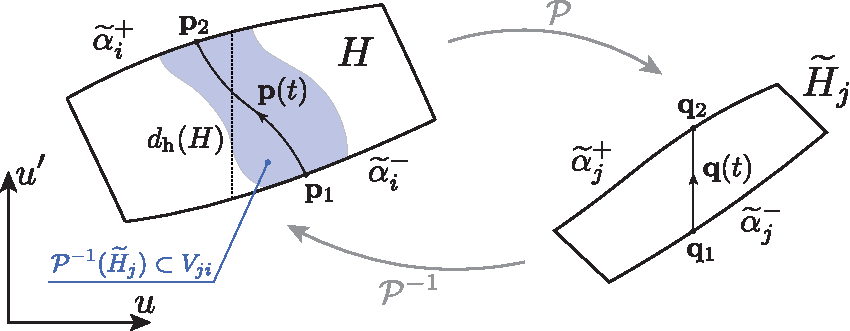
\includegraphics[scale = 1]{pic/thickness of h-strip (a)}
		\caption{
			Illustration for the proof of the h-strips thickness decrease for the case when both h-strips $H$ and $\widetilde{H}_j$ and well-measurable.
			Thickness of $H$ is measured along the vertical dotted line, thickness of $\widetilde{H}_j$ is measured along the vertical line $\vb{q}(t)$.
			Arrows indicate curves traverse directions while $t$ changes from $0$ to $1$.
			Pre-image of $\widetilde{H}_j$ strip is colored with gray.
		}
	\label{fig:thickness-of-h-strip-a}
	\end{figure}
	
	Consider tangent vectors to $\vb{p}(t)$ and $\vb{q}(t)$ (upper dot means the derivative with respect to $t$):
	\begin{eqnarray}
		&& \dot{\vb{p}}(t) = (\dot{\psi}(t), \dot{\psi}'(t)); \\
		&& \dot{\vb{q}}(t) = (0, \dot{\phi}'(t)).
	\end{eqnarray}
	In each point $t$ they are connected by the $D \mathcal{P}_{\vb{p}(t)}$ operator
	\begin{equation}
		\dot{\vb{q}}(t) = D \mathcal{P}_{\vb{p}(t)} (\dot{\vb{p}}(t)).
	\end{equation}
	Rewrite this relation in a matrix form:
	\begin{equation}
		\begin{pmatrix}
			a_{11}(t) & a_{12}(t) \\ a_{21}(t) & a_{22}(t)
		\end{pmatrix}
		\begin{pmatrix}
			\dot{\psi}(t) \\
			\dot{\psi}'(t)
		\end{pmatrix} =
		\begin{pmatrix}
			0 \\ \dot{\phi}'(t)
		\end{pmatrix}.
	\end{equation}
	% TODO: Give a cite, from where follows this fact for Poincar\'e map.
	We take into account that matrix $(a_{mn})$ is a linearization of Poincar\'e map to conclude that its determinant $a_{11}(t) a_{22}(t) - a_{12}(t) a_{21}(t) = 1$ in each point $t$.
	From the relations above and the theorem condition on values of $a_{11}(t)$ follows
	\begin{equation}
		\dot{\phi}'(t) = \dfrac{1}{a_{11}(t)} \dot{\psi}'(t) \le \dfrac{1}{\mu} \dot{\psi}'(t).
	\label{eq:to-integrate}
	\end{equation}
	Integration of \eqref{eq:to-integrate} with limits $0 \le t \le 1$ gives:
	\begin{equation}
		d_{\mathrm{h}}(\widetilde{H}_j) = \phi_2' - \phi_1' = \int \limits_0^1 \dot{\phi}'(t) dt \le \dfrac{1}{\mu} \int \limits_0^1 \dot{\psi}'(t) dt = \dfrac{1}{\mu} (\psi_2' - \psi_1').
	\label{eq:thickness-of-strip-final}
	\end{equation}
	Curve $\vb{p}(t)$ is decreasing and boundaries of $H$ are increasing curves, so it follows from general geometric considerations that $\psi_2' - \psi_1' \le d_{\mathrm{h}}(H)$, i.e. $d_{\mathrm{h}}(\widetilde{H}_j) \le (1 / \mu) d_{\mathrm{h}}(H)$.
	That gives the final statement of the theorem for well-measurable strips.
	
	\begin{figure}[h]
	\centering
		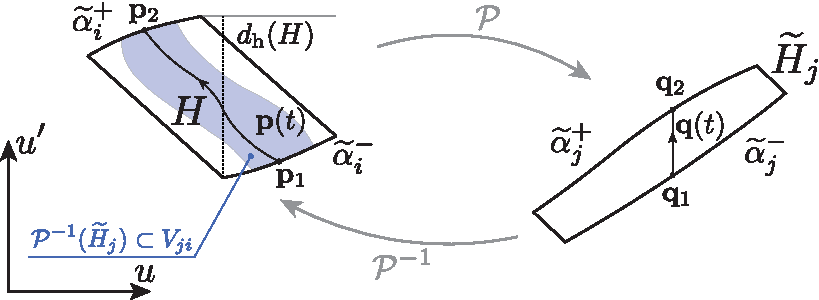
\includegraphics[scale = 1]{pic/thickness of h-strip (b)}
		\caption{
			Illustration for the proof of the h-strips thickness decrease for the case when strip $H$ is not well-measurable.
			Its thickness is measured along the vertical dotted line.
			One endpoint of that line does not belong to the strip boundary $\widetilde{\alpha}_i^+$.
			Pre-image of $\widetilde{H}_j$ strip is colored with gray.
		}
	\label{fig:thickness-of-h-strip-b}
	\end{figure}
	
	The proof above can be easily generalized to the cases when h-strips  $H$ and $\widetilde{H}_j$ are not well-measurable.
	If strip $H$ is not well-measurable, the inequality $\psi_2' - \psi_1' \le d_{\mathrm{h}}(H)$ in \eqref{eq:thickness-of-strip-final} takes place anyway.
	This fact is illustrated on Figure~\ref{fig:thickness-of-h-strip-b}.
	Vertical distance between points $\vb{p}_1, \, \vb{p}_2$ turns out to be certainly less than the width of $H$ strip.
	
	In the case when h-strip $\widetilde{H}_j$ is not well-measurable, one should choose corner points $\vb{q}_1, \, \vb{q}_2$ in a such way that the vertical distance between them equals the thickness of $\widetilde{H}_j$, and then connect $\vb{q}_1, \, \vb{q}_2$ with a monotonic decreasing curve $\vb{q}(t)$, see Fig.~\ref{fig:thickness-of-h-strip-c}.
	This is always possible due to the geometric properties of not well-measurable h-strip.
	According to the choice of points $\vb{q}_1, \, \vb{q}_2$, $d_{\mathrm{h}}(\widetilde{H}_j) = \phi_2 - \phi_1$, and all the steps above remain valid since the corresponding cones mapping with all the consequences can be also applied for the decreasing curves $\vb{p}(t)$ and $\vb{q}(t)$.
	\begin{figure}[h]
	\centering
		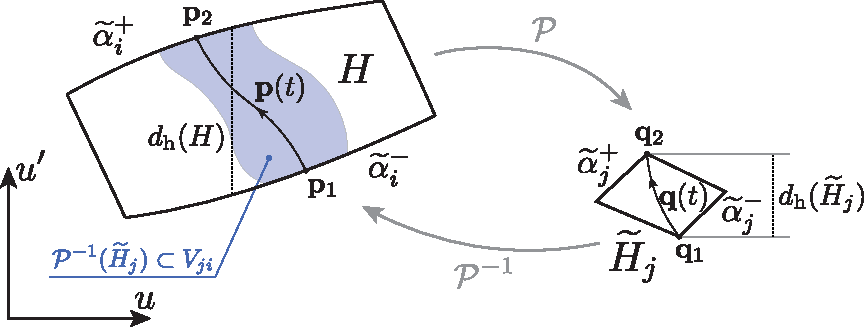
\includegraphics[scale = 1]{pic/thickness of h-strip (c)}
		\caption{
			Illustration for the proof of the h-strips thickness decrease for the case when strip $\widetilde{H}_j$ is not well-measurable.
			Thickness of $H$ and $\widetilde{H}_j$ are measured along the dotted lines.
			Pre-image of $\widetilde{H}_j$ strip is colored with gray.
	  }
	\label{fig:thickness-of-h-strip-c}
	\end{figure}
	
	If both h-strips $H$ and $\widetilde{H}_j$ are not well-measurable then two above mentioned technics should be combined together.
	During the consideration of all other cases of the theorem only type of curves monotonicity is changed, but the overall approach remains the same and can be applied with just minor adjustments.
	Theorem is proven.
\end{proof}

\pagebreak

\begin{theorem}[On v-strips mapping]
\label{thm:v-strips-mapping}
	Let Poincar\'e map $\mathcal{P}$ and its inverse $\mathcal{P}^{-1}$ are defined on a complete (see Definition~\ref{def:complete-island-set}) island set $\bigcup_{i \in S} D_i$, where $S$ is a finite or countable set of indices.
	Let for all $i, j \in S$ set $H_{ij} = \mathcal{P} (D_i) \cap D_j$ is non-empty, $\mathcal{P}^{-1}$ is defined on a
	 closure $\overline{H_{ij}}$, and one of the following two conditions is met:
	\begin{enumerate}
		\item[(1)] borders $\beta_j^{\pm}$ of an island $D_j$ are increasing curves, $\forall \vb{q} \in \overline{H_{ij}}$ signs of values $\{ b_{mn} \}$ in the matrix of the linear operator $D \mathcal{P}_{\vb{q}}^{-1} = (b_{mn})$ have exactly one of the following configurations:
			\begin{center}
				(a) $\begin{psm} + & + \\ + & + \end{psm}$, \quad
				(b) $\begin{psm} - & - \\ - & - \end{psm}$, \quad
				(c) $\begin{psm} + & + \\ - & - \end{psm}$, \quad
				(d) $\begin{psm} - & - \\ + & + \end{psm}$;
			\end{center}
			and at the same time borders $\beta_i^{\pm}$ of $D_i$ are increasing curves for cases (a), (b), and decreasing curves for (c), (d);
		\item[(2)] borders $\beta_j^{\pm}$ of an island $D_j$ are decreasing curves, $\forall \vb{q} \in \overline{H	_{ij}}$ signs of values $\{ b_{mn} \}$ in the matrix of the linear operator $D \mathcal{P}_{\vb{q}}^{-1} = (b_{mn})$ have exactly one of the following configurations:
			\begin{center}
				(a) $\begin{psm} + & - \\ - & + \end{psm}$, \quad
				(b) $\begin{psm} - & + \\ + & - \end{psm}$,	\quad
				(c) $\begin{psm} + & - \\ + & - \end{psm}$, \quad
				(d) $\begin{psm} - & + \\ - & + \end{psm}$;		
			\end{center}
			and at the same time borders $\beta_i^{\pm}$ of $D_i$ are decreasing curves for cases (a), (b), and increasing for (c), (d);
	\end{enumerate}
	and moreover $\exists \nu > 1$ such that $\forall q \in \overline{H_{ij}}$, $|b_{22}| \ge \nu$, then for any \emph{v}-strip $V \in D_j$, $\mathcal{P}^{-1} (V) \cap D_i = \widetilde{V}_i$ is also a \emph{v}-strip, and $d_{\mathrm{v}} (\widetilde{V}_i) \le (1 / \nu) d_{\mathrm{v}} (V)$ (here $d_{\mathrm{v}}(\cdot)$ is an \emph{v}-strip thickness in a sence of Definition~\ref{def:v-thickness}).
\end{theorem}
\begin{proof}
	Completely analogous to the proof of the h-strips mapping theorem.
\end{proof}

% Bibliography
\printbibliography[heading=bibintoc]

% Appendix
% \appendix
% \input{a}

\end{document}
